
\documentclass[
  10pt % font size
  16:9, % 1920x1080
]{beamer}
% \usetheme{default}
% \usetheme{Boadilla}
 \usetheme{Madrid}
% \usetheme{Montpellier}
% \usetheme{Warsaw}
% \usetheme{Copenhagen}
% \usetheme{Goettingen}
% \usetheme{Hannover}
% \usetheme{Berkeley}
\usepackage{booktabs}
 
% \usecolortheme{crane}
 % \beamertemplatesolidbackgroundcolor{craneorange!25}
 
 % Define custom colors
\definecolor{customGreen}{RGB}{0,128,0} % A medium green
\definecolor{customDarkGreen}{RGB}{0,100,0} % A darker green

\usepackage{hyperref}

% Apply the custom colors
\usecolortheme{default} % Start with the default color theme to apply custom colors on top
\setbeamercolor{structure}{fg=customGreen}
\setbeamercolor{background canvas}{bg=white} % Set main background to white
\setbeamercolor{title}{bg=customDarkGreen,fg=white} % Title slide background
\setbeamercolor{frametitle}{bg=customGreen,fg=white} % Frame titles

% Custom footline with an image on the bottom right
\addtobeamertemplate{footline}{}{%
  \hfill%
  \raisebox{5mm}[0pt][10pt]{%
  
\includegraphics[height=1cm]{kyu_univ_logo.png}%
  }\hspace*{5mm}
}

\title{Article Classification with Centroid Classification}
\subtitle{}

\author{Group 1}

\date[June 19, 2024]
 {June 19, 2024}

\begin{document}

\frame{\titlepage} % # 1
\section[Outline]{}
\frame{\tableofcontents}

\section{Project Overview}
 
\frame % # 2
{
  \frametitle{Project Objectives}
  \begin{itemize}
  \item The goal of this project is classify document per category on given dataset.
  \item Document Embedding Model: Tf-Idf Vectorizer
  \item Classification Model: Centroid Classification
  \end{itemize}
}

\section{Dataset and Pre-liminary Analysis}
\frame
{
  \frametitle{Dataset and Pre-liminary Analysis}
  \begin{itemize}
  \item \href{http://mlg.ucd.ie/datasets/bbc.html}{BBC ML Dataset}
  \item Consist of 2225 articles, with categories: 'business', 'entertainment', 'politics', 'sport', 'tech'
  \item Dataset was changed from Wikipedia to BBC dataset due to complication in model training and dataset processing.
  \end{itemize}
  \begin{figure}
  \centering
  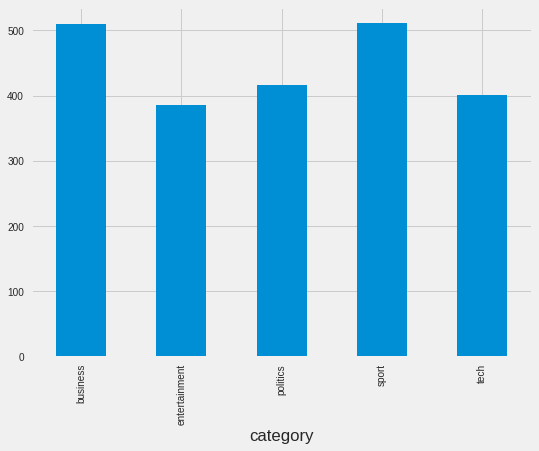
\includegraphics[width=0.5\textwidth]{categories.png}
  \end{figure}
}

\section{Data Preprocessing}
\frame
{
  \frametitle{Data Preprocessing}
  \begin{itemize}
  \item Category-Token Chi2 test
  \end{itemize}
  \begin{table}
  \centering
  \begin{tabular}{@{}llllll@{}}
    \toprule
    Category       & 1st       & 2nd      & 3rd      \\ \midrule
    Business       & oil       & bank     & growth   \\
    Entertainment  & award     & singer   & awards   \\
    Politics       & tory      & blair    & party    \\
    Sport          & win       & injury   & coach    \\
    Tech           & digital   & computer & software \\
    \bottomrule
  \end{tabular}
  \end{table}
}

\begin{frame}
  \frametitle{Tf-Idf Embedding}
  \begin{itemize}
  \item We use tf-idf scoring to encode the documents.
  \item The token value is calculated as follows:
  \begin{align}
    tf(t,d) &= \frac{f_{t,d}}{\sum_{t' \in d} f_{t',d}} \\
    idf(t) &= \log\left(\frac{N}{n_t}\right) \\
    tfidf(t,d) &= tf(t,d) \times idf(t)
  \end{align}
  \end{itemize}
\end{frame}

\begin{frame}
  \frametitle{Tf-Idf Embedding}
  \begin{itemize}
  \item Prior to embedding, unique words(unigrams and bigrams) are extracted from the dataset to be used as tokens. Each token is associated with token index which will be used as vector index.
    \item For each document, the token value(vector index) in the vector is given by tf-idf scoring of document.
  \end{itemize}
\end{frame}

\section{Centroid/Variance Calculation}
\begin{frame}
  \frametitle{Document Vectorization and Clustering}
  \begin{itemize}
    \item With the documents embedded, we now calculate the centroid and variance of each categories.
    \item Centroid is the main metric for the cluster, and variance is calculated to use gaussian distribution for probability distribution.
    \item No dimension reduction is applied to minimize information loss.
    \item We evaluate the model on normalized dataset and non-normalized dataset. For normalized dataset, we use distance matric $\frac{1}{\cos(\theta)}$, where $\cos(\theta)$ is the cosine similarity, and for non-normalized dataset, we use euclidean distance.
  \end{itemize}
\end{frame}

\begin{frame}
  \frametitle{Centroid Classification}
  \begin{itemize}
    \item Centroid classification is a simple classification method that uses the centroid and distance metric to classify the document.
    \item Our project uses method: Nearest Centroid, Gaussian Probability Distribution, and Logistic function.
    \item The category prediction is generated by calculating highest score of probability distribution, or lowest distance from the centroid.
  \end{itemize}
\end{frame}

\begin{frame}
  \frametitle{Nearest Centroid}
  \begin{itemize}
    \item The simplest centroid classification method, where the document is classified based on the nearest centroid.
    \item The distance metric is calculated using the distance metric, and the document is classified based on the nearest centroid.
    \item The centroid is calculated as the mean of the document vectors in the cluster.
  \end{itemize}
\end{frame}

\begin{frame}
  \frametitle{Gaussian Probability Distribution}
  \begin{itemize}
    \item For each unique category, we construct a probability distribution using the centroid of the cluster and distance metric.
    \item Assuming central-limit theorem, we use a normal distribution to generate the probability distribution.
    \[
      p(d) = \frac{1}{\sqrt{2\pi}\sigma}e^{-\frac{(d)^2}{2\sigma^2}}
    \]
    Where d is the distance from the centroid, and \(\sigma\) is the variance of the cluster.
  \end{itemize}
\end{frame}

\begin{frame}
  \frametitle{Logistic Function}
  \begin{itemize}
    \item Use Logistic Function to smooth the distance metric.
    \[
      p(d) = \frac{1}{1+e^{-\alpha d}}
    \]
    Where d is the distance from the centroid. We use $\alpha$ as a hyperparameter to tune the distribution, and it's set to 0.5.
  \end{itemize}
\end{frame}

\begin{frame}
  \frametitle{Multi-Category Classification}
  \begin{itemize}
    \item For multi-category classification, we use the probability distribution to predict the category of the document.
    \item We can tune the probability threshhold for accuracy using the cost function:
    \[
      J(C_d, C_d') = \frac{\lambda_1|C_d'\setminus C_d| + \lambda_2|C_d\setminus C_d'|}{|C_d\cup C_d'|}
    \]
    where $C_d$ is document categories set, and $C_d'$ is predicted categories set.
    \item Starting from threshold 0, we increase the threshold by a learning rate value until the cost function is minimized.
    \item We generate a candidate category for both pmf value using trained threshold, and choose candidate of which have same candidate for Gaussian and Logistic.
  \end{itemize}
\end{frame}

\begin{frame}
  \frametitle{Evaluation}
  \begin{itemize}
    \item Model Accuracy
  \end{itemize}
  \begin{table}
    \centering
    \begin{tabular}{@{}llllll@{}}
        \toprule
        Category       & Accuracy\\ \midrule
        Closest Centroid       & 0.95\\
        Closest Centroid Normalized  & 0.97\\
        Gaussian       &0.34 \\
        Gaussian Normalized          &0.93 \\
        Logistic           &0.95 \\
        Logistic Normalized           &0.97 \\
        \bottomrule
    \end{tabular}
  \end{table}
\end{frame}

\begin{frame}
  \frametitle{Evaluation}
  \begin{figure}
    \centering
    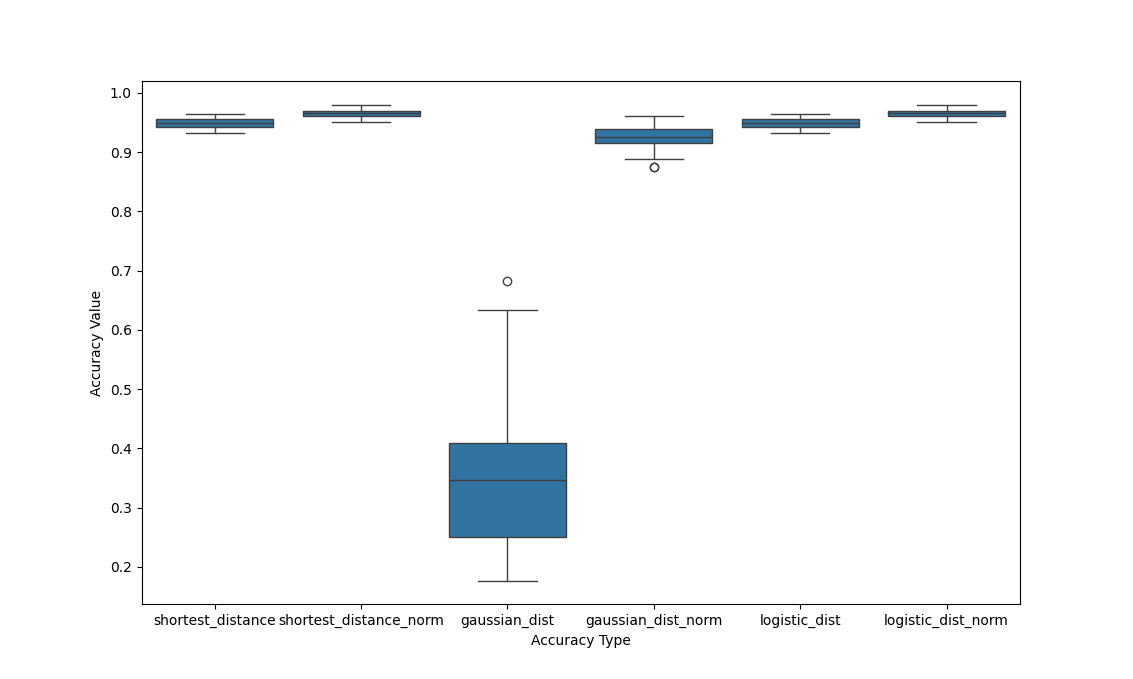
\includegraphics[width=1\textwidth]{error_map.png}
  \end{figure}
\end{frame}

\begin{frame}
  \frametitle{Multiple Category Classification}
  \begin{figure}
    \centering
    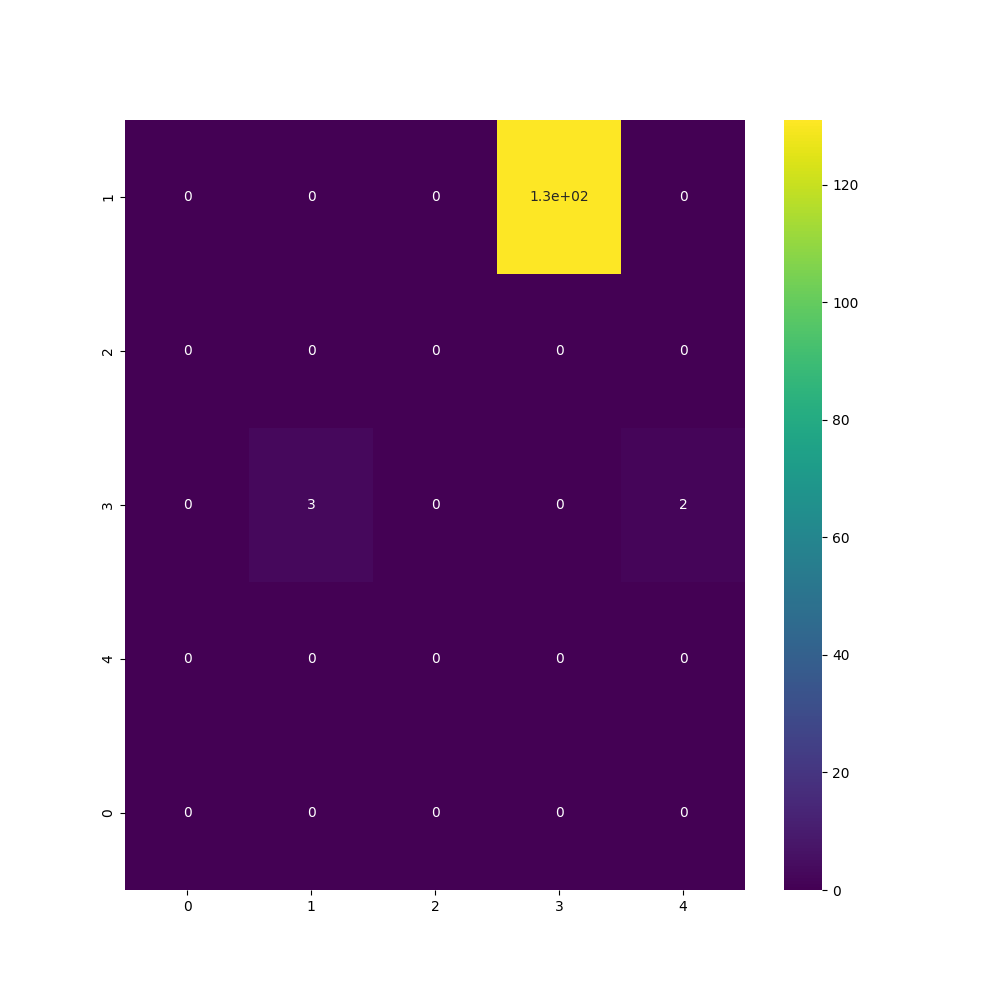
\includegraphics[width=0.6\textwidth]{candidate_relation.png}
  \end{figure}
\end{frame}

\begin{frame}
  \frametitle{Multiple Category Classification[Normalized Dataset]}
  \begin{itemize}
    \item Sports article were most associated with entertainment, while entertainment article was candidate for only 3 sports. The 3 documents commonly include description of winning an award or similar context
    \item 1 tech documents were incorrectly labled as sports, which included description of video game metal slug.
  \end{itemize}
\end{frame}

\begin{frame}
  \frametitle{Entertainment with Candidate Sports}

Ray's success on DVD outstripped its \$74m (£40m) US box office total, earning more than \$40m (£22m) on the first day of the DVD's release alone. Ray has been nominated in six Oscar categories including best film and best actor for Jamie Foxx. The film recounts the life of blues singer Ray Charles, ...
\end{frame}

\begin{frame}
  \frametitle{Miscategorized Tech Article}
Like some drill sergeant from the past, Metal Slug 3 is a wake-up call to today's gamers molly-coddled with slick visuals and fancy trimmings.

With its hand-animated sprites and 2D side-scrolling, this was even considered retro when released in arcades four years ago. But a more frantic shooter you will not find at the end of your joypad this year. And yes, that includes Halo 2. Simply choose your grunt and wade through five 2D side-scrolling levels of the most hectic video game blasting you will ever encounter. It is also the toughest game you are likely to play, as hordes of enemies and few lives pile the pressure on...
\end{frame}
\end{document}